%!TEX root = ../thesis.tex
\chapter{Zero Knowledge Proofs}
\label{zkp}

A proof of knowledge is a protocol that enables one party to convince another of the validity of a statement.
In a zero-knowledge proof, this is accomplished without revealing any information beyond the legitimacy of the proof~\cite{kiagias:crypto},
meaning that one party can prove to another party that a given statemnet is true, without conveying any information apart from
the fact that the statement is indeed true~\cite{wiki:zkp}.

Let $\calp$ be a prover and $\calv$ the verifier. $\calp$ must convince $\calv$ that she has some
knowledge of a statement $x$ without explicitly stating what she knows. We call this knowledge a witness $w$.
Both parties are aware of a predicate $R$ that will attest to $w$ being a valid witness to $x$~\cite{kiagias:crypto}. In general,

\begin{itemize}
  \item The predicate $R$ is assumed to be polynomial-time computable.
  \item The prover $\calp$ has $R,x$, and $w$ such that $R(x,w) = 1$. She wishes to prove possesion of $w$ by producing a proof of knowledge $\pi$.
  \item The verifier $\calv$ has $R,x$, and $\pi$.
  \item Given $R$ it is hard to find a corresponding $w$ such as $R(x,w) = 1$
  \item The prover $\calp$ is reluctant to reveal $w$; otherwise the solution is trivial.
  \item The verifier $\calv$ can efficiently check the validity of $\pi$.
\end{itemize}

\section{Examples}

\subsection{The strange cave of Ali Baba}
\label{zkp:examples}

Suppose there is our old friends Alice and Bob. At the bottom of the cave~\cite{Quisquater:1989:EZP:118209.118269} of figure~\ref{fig:zkp:alibaba} there is a magic door that
can only be open using a secret password. The cave is shaped like a rentacle with one entrace at one side and the magic door blocking the opposite side.
Bob knows the secret password and wants to prove to Alice that he can open the magic door without revealing the password to Alice.
Bob propose the following game to prove to Alice he can open the magic door: Alice waits outside the cave, Bob enters the cave and
takes either left or right path. Alice can not see which path Bob takes. Then Alice enters, stants at the entrance of cave and calls
Bob to come out either the left or the right passage. Bob complies, using the secret password if necessary.

If Bob does not know the secret password he has $1/2$ change of guessing correctly (he would only be able to return by the named path if
Alice were to give the name of the same path by which he had entered) as Alice choose at random which path Bob should take. If they repeat this procedure
$k$ times the probability of Bob convincing Alice that he knows the secret password without actually knowing it reduce exponetially. In particular, at most $1/2^{k}$.

\subsection{The colour-blind friend}

Let's bring again our friends Alice and Bob. Suppose Bob is color-blind~\cite{wiki:zkp,zkp:colour_blind} and Alice has two balls: one red and one green but otherwise identical when you touch them.
To Alice they seem complete identical and she is not sure if they are actually distinguishable. Bob wants to prove to Alice that indeed the are differently-coloured
without revealing which one is red and which is green. To prove his knowledge, Bob gives to Alice the two balls so that she is holding one in each hand. Bob can see
at this point which ball is in which hand. Next, Alice either switches the ball behind her hands or leaves them be, with probability $1/2$. Finally, she brings
them out from behind her back. Alice then asks Bob if she switch the balls. By looking at their colors, Bob can can say with certainty whether he switched them or not.
On the other hand, if they were the same color and hence indistinguishable, there is no way you could guess correctly with probability higher than 1/2. If they repeat
this procedure $k$ times the probability that Bob succeeded at identifying all the switch/non-switches when the balls are identical (thus lying to Alice) is at most
$1/2^{k}$.

\begin{figure}[t!]
  \centering
  \begin{subfigure}[t]{0.30\textwidth}
    \centering
    \resizebox{\linewidth}{!}{
      \begin{tikzpicture}[scale=1]
        % Cave %
        \draw(0,5) -- (2,5) -- (2,8) -- (10,8) -- (10,4);
        \draw(0,4) --(2,4) -- (2,1) -- (10,1) -- (10, 4);
        \draw(9,4.5) -- (10,4.5);
        \draw(3,5) -- (3,7) -- (9,7) -- (9,5);
        \draw(3,5) -- (3,2) -- (9,2) -- (9,5);
        % Actors %
        \draw[fill] (1,5.6) circle [radius=0.1];
        \node [below] (alice) at (1,5.5) {Alice};
        \draw[fill] (2.5,4.6) circle [radius=0.1];
        \node [below] (bob) at (2.5,4.5) {Bob};
        % Arrows %
        \draw [dashed, ->] (2.5,4.6) -- (2.5,6);
        \draw [dashed, ->] (2.5,3.9) -- (2.5,2);

      \end{tikzpicture}
    }
    \caption{Alice stands outside and Bob choose randomly a path, left or right}
    \label{fig:zkp:alibaba:a}
  \end{subfigure}
  \begin{subfigure}[t]{0.30\textwidth}
    \centering
    \resizebox{\linewidth}{!}{
      \begin{tikzpicture}[scale=1]
        % Cave %
        \draw(0,5) -- (2,5) -- (2,8) -- (10,8) -- (10,4);
        \draw(0,4) --(2,4) -- (2,1) -- (10,1) -- (10, 4);
        \draw(9,4.5) -- (10,4.5);
        \draw(3,5) -- (3,7) -- (9,7) -- (9,5);
        \draw(3,5) -- (3,2) -- (9,2) -- (9,5);
        % Actors %
        \draw[fill] (2.5,4.6) circle [radius=0.1];
        \node [below] (alice) at (2.5,4.5) {Alice};
        \draw[fill] (9.5,4.3) circle [radius=0.1];
        \node [below] (bob) at (9.5,4.2) {Bob};
        % Speech Bubble %
        \node[overlay,draw,cloud callout,callout relative pointer={(0.2cm,-0.7cm)},%
        aspect=2.5,fill=white!90] at ($(alice)+(-0.5cm,2.3cm)$) {Left};

      \end{tikzpicture}
    }
    \caption{Alice calls to Bob, asking him to come out either the left or the right passage}
    \label{fig:zkp:alibaba:b}
  \end{subfigure}
  \begin{subfigure}[t]{0.30\textwidth}
    \centering
    \resizebox{\linewidth}{!}{
      \begin{tikzpicture}[scale=1]
        % Cave %
        \draw(0,5) -- (2,5) -- (2,8) -- (10,8) -- (10,4);
        \draw(0,4) --(2,4) -- (2,1) -- (10,1) -- (10, 4);
        \draw(9,4.5) -- (9.5,4.5);
        \draw(3,5) -- (3,7) -- (9,7) -- (9,5);
        \draw(3,5) -- (3,2) -- (9,2) -- (9,5);
        % Actors %
        \draw[fill] (2.5,4.6) circle [radius=0.1];
        \node [below] (alice) at (2.5,4.5) {Alice};
        \draw[fill] (2.5,7.8) circle [radius=0.1];
        \node [below] (bob) at (2.5,7.7) {Bob};
        % Speech Bubble %
        \node[overlay,draw,cloud callout,callout relative pointer={(0.2cm,-0.7cm)},%
        aspect=2.5,fill=white!90] at ($(alice)+(-0.5cm,2.3cm)$) {OK};

      \end{tikzpicture}
    }
    \caption{Bob complies appearing at the exit Alices names}
    \label{fig:zkp:alibaba:c}
  \end{subfigure}
  \caption{Ali Baba Cave}
  \label{fig:zkp:alibaba}
\end{figure}

\section{Formal Definition}
\label{zkp:definition}

Let $<\calp, \calv>$ be a pair of interactive programs. Define $\text{out}^{\calp}_{\calp, \calv}(x,w,z)$
to be the output of $\calp$ when both $\calp$ and $\calv$ are executed with the public input $x$ and private
inputs $w$ and $z$ ($\calp$ determines $w$ and $\calv$ choose $z$); $\text{out}^{\calv}_{\calp, \calv}(x,w,z)$
is similar defined for $\calv$. The PPT interactive protocol $<\calp, \calv>$ is a \textbf{zero-knowledge proof}
for a language $L \in NP$ with knowledge error $k$ and zero-knowledge distance $\e$ if the following
properties hold~\cite{kiagias:crypto}.

\begin{enumerate}
  \item \textbf{Completeness:} If $x \in L$ and $R(x,w) = 1$ for some witness $w$, then $\text{out}^{\calv}_{\calp, \calv}(x,w,z)$ = 1
    for all string $z$ with overwhelming probability in $v$.
  \item \textbf{Soundness:} For any polynomial-time program $\calp^{*}$ define for arbitrary $x,w,z,$
    \begin{equation*}
      \pi_{x,w,z} = \Prob[\text{out}^{\calv}_{\calp^{*}, \calv}(x,w,z) = 1].
    \end{equation*}
    A protocol $<\calp, \calv>$ satisfies soundness if there are non-negligible functions $s(v), q(v)$ such for all $\calp^{*}$ here exists a probabilistic
    Turing machine (PTM) program $K$, called a knowledge extractor with the following property. Suppose that

    \begin{equation*}
      \widetilde{\pi} = \Prob[K(x,w,z) = w^{'} : R(x, x^{'}) = 1].
    \end{equation*}
    Then it holds that $\pi_{x,w,z} \geq s(|x|)$ implies that $\widetilde{\pi}_{x,w,z} \geq q(\abs{x})$.

  \item \textbf{(Statistical) Zero-knowledge:} For each polynomial-time program $\calv^{*}$, there is a PTM program $S$, called the \textbf{simulator}, such that for all
    $x,w$ with $R(x,w) = 1$, the random variables $S(x,z)$ and $\text{out}^{\calv^{*}}_{\calp, \calv^{*}}(x,w,z)$ are statistically indistinguishable for all strings $z$:
    \begin{equation*}
      \forall \cala \abs[\Big]{\Prob[\cala(S(x,z) = 1)] - \Prob[\cala(\text{out}^{\calv^{*}}_{\calp, \calv^{*}}(x,w,z)) = 1]} < \e.
    \end{equation*}
\end{enumerate}

Completeness is very similar to correctness. Assuming both the prover and verifier follow the protocol faithfully, completeness guarantees that the
protocol will succeed with a sufficiently high probability.
Soundness ensures that if the statement is false, no cheating prover can convince the honest verifier that it is true, except with some small probability.
Intuitively, statistical zero-knowledge is a property that prohibits a verifier from extracting information from an honest prover.
A weaker version of zero-knowledge is honest-verifier zero-knowledge (HVZK). Here it is assumed that the verifier executes the protocol faithfully,
but makes additional computations~\cite{kiagias:crypto}.

\section{zk-SNARKs}
\label{zkp:snarks}

Since computational power is often limited to devices such as mobiles or IoT (clients) the need of outsourcing computation to one or more powerful workers on the cloud emerges. Yet, confidence is needed at the working entity for proper computation. For this reason, the client should be able to verify the correctness of the results returned. That way not only the client is protected from malicious or malfunctioning workers but also the legitimate worker is benefit by shedding liability~\cite{pinocchio-nearly-practical-verifiable-computation}. This scheme is called public verifiable computation (VC).

In a public verifiable computation scheme the client outsource the evaluation of a function $F$ on input $u$ known to the client (e.g. a query). The client then can verify the correctness of the computation of $F(u)$ with less work than required for the computation of $F(u)$. When the outsource function $F$ consist of two inputs $u$ and $w$, where $w$ is the worker's private input (e.g a data set), then the scheme is a Zero-Knowledge Verifiable Computation (or non-interactive zero knowledge (NIZK) proof~\cite{Blum:1991:NZ:123137.123145}) if the client learns nothing about worker's input expect the output of the computation~\cite{pinocchio-nearly-practical-verifiable-computation}.

Such schemes are not interactive meaning no interaction is necessary between prover and verifier (worker and client) and a common reference string (CRS) shared between them is enough to achieve computational zero-knowledge~\cite{Blum:1991:NZ:123137.123145}.

Formally, as defined by Parno et. al~\cite{pinocchio-nearly-practical-verifiable-computation} a public Zero-Knowledge verifiable computation scheme $\calv \calc$ consist of a set of three polynomial-time algorithms:

\begin{itemize}
  \item $(EK_F, VK_F) \leftarrow \text{KeyGen}(F, 1^{\lambda})$: The randomized key generation algorithm. It takes as input the outsourced function $F$ and a security parameter ${\lambda}$; it outputs a public evaluation key $EK_F$ and a public verification key $VK_F$.
  \item $(y, \pi_y) \leftarrow \text{Compute}(EK_F, u)$: The deterministic worker algorithm. It takes as input the public evaluation key $EK_F$ and a public input $u$; it outputs $y \leftarrow F(u, w)$, where $w$ is an auxiliary private input, and a proof $\pi$ of $y$'s correctness.
  \item $\{0, 1\} \leftarrow \text{Verify}(VK_F, u, y, \pi_y)$:  The deterministic verification algorithm. It takes as input the public verification key $VK_F$, the public input $u$, the output $y$ and the proof $\pi_y$; It outputs $1$ if $F(u) = y$ and $0$ otherwise.
\end{itemize}

The acronym zk-SNARK stands for `Zero-Knowledge Succinct Non-Interactive Argument of Knowledge` in which each individual part, informally, have the following meaning~\cite{zksnarks_nutshell, zcash, 184425, Bitansky:2012:ECR:2090236.2090263}:

\begin{itemize}
  \item Zero-Knowledge: The verifier learns nothing but the validity of the computation
  \item Succinct: The proof are sort and easy to verify in comparison to the actual computation (constant size and polynomial verifiable in the size of the proof)
  \item Non-Interactive: There is no or little interaction done in one step. Anyone can verify without the need of interacting anew (publicly verifiable)
  \item ARgument: Soundness (§~\ref{zkp:definition}) holds only against computationally bounded provers
  \item of Knowledge: If the verifier accepts a proof output by a computationally bounded prover, then the prover has a witness for the given instance
\end{itemize}

At high level, zkSNARKs consist of four basic steps (Figure ~\ref{fig:zkp:zksnark_flow}):

\begin{enumerate}
  \item Computation to Arithmetic circuit~\cite{wiki:circuits}
  \item Arithmetic circuit to Rank 1 Constraint System (R1CS)~\cite{ggpr}
  \item R1CS to Quadratic Span Program (QAP)~\cite{ggpr}
  \item QAP to zkSNARK~\cite{pinocchio-nearly-practical-verifiable-computation}
\end{enumerate}

The main idea for constructing zkSNARKs is firstly to transform the generic program as a quadratic equation of polynomials (QAP)~\cite{ggpr}: $p(x)q(x) = s(x)r(x)$, where the equality holds if and only if the program is computed correctly. So the prover wants to convince the verifier that the equality holds.

Succinctness is achieved by random sampling. The verifier chooses a secret evaluation point $x_0$ to reduce the problem from polynomial multiplication and equality to simple number arithmetic checks: $p(x_0)q(x_0) = s(x_0)r(x_0)$. To allow the prover to compute the evaluation of the polynomials at $x_0$, without revealing $x_0$, Homomorphic encryption is used:  $E(p(x_0))E(q(x_0)) = E(s(x_0))E(r(x_0))$

Finally the prover obfuscates the encrypted values by multiplying with a number so that the verifier can still check the correctness of the structure without knowing the actual
encrypted values: $E(k + p(x_0))E(k + q(x_0)) = E(k + s(x_0))E(k + r(x_0))$

\begin{figure}[ht!]
  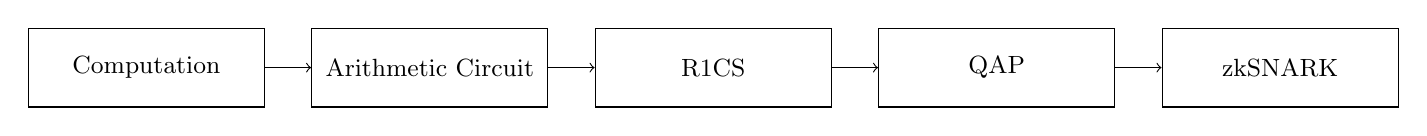
\begin{tikzpicture}[
    flow/.style={rectangle, minimum width=3cm, minimum height=1cm, text centered, draw=black,font=\small},
    scale=0.9
  ]
    \node[flow] (comp) at (0, 0) {Computation};
    \node[flow] (alg) at (4, 0) {Arithmetic Circuit};
    \node[flow] (r1cs) at (8, 0) {R1CS};
    \node[flow] (qap) at (12, 0) {QAP};
    \node[flow] (zk) at (16, 0) {zkSNARK};

    \draw[->] (comp) -- (alg);
    \draw[->] (alg) -- (r1cs);
    \draw[->] (r1cs) -- (qap);
    \draw[->] (qap) -- (zk);


  \end{tikzpicture}
  \caption{Steps of zk-SNARK}
  \label{fig:zkp:zksnark_flow}
\end{figure}

\note{Implementations of zksnark (pinnochio, Hawk, Zcash etc)}
